% 3-minute talking-point deck boiled down from ../report/yolo_report.pdf (18 Nov 2026).
% Self-contained: no \input, all numbers inline. Build: tectonic yolo_talk.tex
\documentclass[aspectratio=169,11pt]{beamer}
\usetheme{default}
\setbeamertemplate{navigation symbols}{}
\setbeamertemplate{footline}{\hfill\scriptsize\color{muted}\insertframenumber/\inserttotalframenumber\hspace{6pt}\vspace{4pt}}
\usepackage[T1]{fontenc}
\usepackage{lmodern}
\usepackage{booktabs}
\usepackage{pgfplots}
\pgfplotsset{compat=1.18}
\definecolor{vec}{HTML}{2A78D6}
\definecolor{scal}{HTML}{EB6834}
\definecolor{his}{HTML}{8A5CC2}
\definecolor{muted}{HTML}{6B6A64}
\definecolor{gridc}{HTML}{E4E3DE}
\setbeamercolor{frametitle}{fg=black}
\setbeamercolor{structure}{fg=vec!80!black}
\setbeamerfont{frametitle}{series=\bfseries, size=\large}
\newcommand{\iss}[1]{\href{https://github.com/JieGH/RVV_code_gen_via_MLIR_xDSL/issues/#1}{\##1}}
\newcommand{\src}[1]{\par\vfill{\tiny\color{muted}#1\par}}
\newcommand{\say}[1]{{\small\color{muted}\emph{Say:} #1}}

\title{YOLO GEMM on the SpacemiT K1}
\subtitle{Best microkernel sizes, ours against H\'ector's, and why we trail at 1 thread}
\date{18 Nov 2026 \quad$\cdot$\quad 3-minute summary of the combined YOLO report (\iss{58})}

\begin{document}

% ---------------------------------------------------------------- 0:00-0:20
\begin{frame}
\titlepage
\vfill
{\scriptsize\color{muted}
\textbf{Terms.} \emph{GOPs by mean time}: $2mnk \div$ mean time per call (all numbers).
\emph{ms per pass}: one call per YOLO shape, summed (50 shapes).
\emph{Launch}: one full run; 3 launches per side, A-B-B-A order.
\emph{Tile MR$\times$NR}: the microkernel's block of C.
\emph{1T}: 1 thread on core 4; \emph{8T}: cores 0--7, threads bound.
Uninstrumented build, reference protocol, idle jbpi, \texttt{--no-nc-overrides}.\par}
\end{frame}

% ---------------------------------------------------------------- 0:20-1:00
\begin{frame}{1. H\'ector's ask: which microkernel sizes run fastest?}
\begin{itemize}
\item \textbf{1 thread: 24x8} for the whole network.\\
  698.6\,ms per pass (4.26 GOPs) vs.\ 785.3\,ms (3.79 GOPs) at H\'ector's 16x8.
\item \textbf{8 threads: a family, chosen by $n$}
  \begin{itemize}
  \item $n \le 8$: MR\,32 / NR\,4 \quad $n = 16$--$64$: MR\,32 / NR\,6--7 \quad $n \ge 80$: MR\,16 / NR\,12--15
  \item Best tile per shape \textbf{134.1\,ms}; best single tile (16x12) 145.6\,ms; 16x8 149.6--149.8\,ms
  \end{itemize}
\item The best tile at 1T is not the best at 8T (also true for the paper shapes).
\end{itemize}
\vspace{4pt}
\say{pick the tile by $n$ at 8T; about 10\% off the pass vs.\ 16x8 --- but timed in \emph{our} GEMM, not H\'ector's.}
\src{Report Part 1 (\iss{61}--\iss{63}, \iss{82}). 19 candidate tiles per shape.}
\end{frame}

% ---------------------------------------------------------------- 1:00-1:40
\begin{frame}{2. Our GEMM against H\'ector's, one mixed series (\iss{94})}
\begin{columns}[T]
\begin{column}{0.52\textwidth}
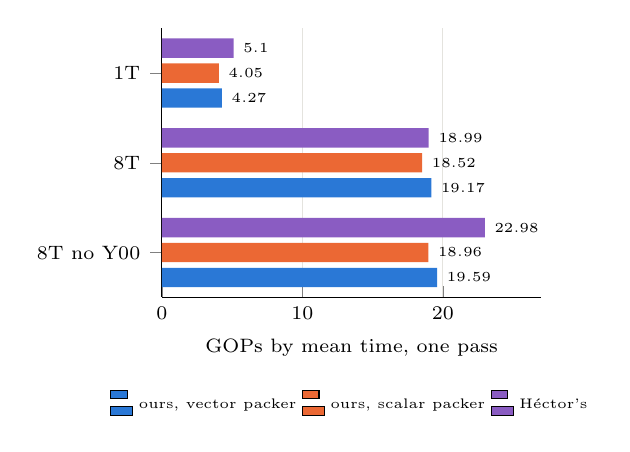
\begin{tikzpicture}
\begin{axis}[xbar, width=6.4cm, height=5.0cm, y dir=reverse, xmin=0, xmax=27,
  symbolic y coords={1T,8T,8T no Y00}, ytick=data, enlarge y limits=0.25,
  bar width=7pt, axis x line*=bottom, axis y line*=left,
  xmajorgrids, grid style={gridc}, tick label style={font=\scriptsize},
  xlabel={GOPs by mean time, one pass}, label style={font=\scriptsize},
  nodes near coords, every node near coord/.append style={font=\tiny},
  legend style={font=\tiny, draw=none, at={(0.5,-0.32)}, anchor=north, legend columns=3}, legend cell align=left]
\addplot[fill=vec, draw=none]  coordinates {(4.27,1T) (19.17,8T) (19.59,8T no Y00)};
\addplot[fill=scal, draw=none] coordinates {(4.05,1T) (18.52,8T) (18.96,8T no Y00)};
\addplot[fill=his, draw=none]  coordinates {(5.10,1T) (18.99,8T) (22.98,8T no Y00)};
\legend{{ours, vector packer}, {ours, scalar packer}, {H\'ector's}}
\end{axis}
\end{tikzpicture}
\end{column}
\begin{column}{0.46\textwidth}
\begin{itemize}
\item \textbf{1T:} H\'ector's 5.10 vs.\ ours 4.27 GOPs.
\item \textbf{8T, whole pass:} tie --- 19.17 vs.\ 18.99, inside the launch range.
\item \textbf{8T without Y00:} H\'ector's leads, 22.98 vs.\ 19.59. His Y00 is slow and unstable (29.5--30.4\,ms vs.\ ours 6.7--7.4).
\end{itemize}
\vspace{4pt}
\say{at the same tile, his engine is about 15\% faster. We need to close the 1T gap.}
\end{column}
\end{columns}
\src{Ours at tile 24x8; H\'ector's gemm.bin at b292c92, his tiles, TIMIN=2.0. Compilers differ: ours g++ 13.2 -O2, his gcc-14 -O3.}
\end{frame}

% ---------------------------------------------------------------- 1:40-2:20
\begin{frame}{3. Why we trail at 1 thread: the A packer's read order (\iss{95})}
\begin{itemize}
\item A is stored column by column.
  \begin{itemize}
  \item \textbf{Ours:} one 24-row panel at a time; jumps a full column per read (19.2\,KB on Y10).
  \item \textbf{H\'ector's:} reads each column once, top to bottom. Same bytes, same packed result.
  \end{itemize}
\item The pack is \textbf{77\%} of our time on Y10 and \textbf{90\%} on Y05.\\
  Our compute alone on Y10: about 7.8 GOPs --- faster than his whole call (5.1).
\item The gap sits on large $m$, small $k$: \textbf{131.0 of 140.5\,ms} on 23 shapes with $m>300$, $k \le kc$.\\
  A board pack test puts the read-order cost at 162.2\,ms --- the same size.
\item Not the cause: block size along $m$, or the 24x8 microkernel.
\end{itemize}
\say{the kernel is fine; the packer reads A in the wrong order. Fix: pack A column by column (\iss{96}).}
\src{Pack shares from the instrumented build (shares only). Pack test: \texttt{issue95/pack\_order.c} on jbpi; gives the size of the order effect, not exact times.}
\end{frame}

% ---------------------------------------------------------------- 2:20-2:45
\begin{frame}{4. Paper shapes and packing}
\begin{itemize}
\item \textbf{Paper BERT/Square (\iss{71}):}
  1T --- the paper's 32x7 holds (wins 9 of 10 shapes).
  8T --- it does not: 16x8 wins 8 of 10 and the pass (48.27 vs.\ 44.07 GOPs).
\item \textbf{Packing (\iss{83}, \iss{85}): keep the vector packer.}
  \begin{itemize}
  \item YOLO, scalar $\div$ vector GOPs: median 0.929 (1T), 0.945 (8T); down to 0.58 at $n=4$.
  \item Slowdown $\approx$ pack share $\times$ extra pack cost; small $n$ means a large pack share.
  \end{itemize}
\end{itemize}
\src{Report Parts 2--3. BERT/Square from Table 1 of arXiv 2603.17800v1.}
\end{frame}

% ---------------------------------------------------------------- 2:45-3:00
\begin{frame}{5. Next}
\begin{enumerate}
\item \textbf{\iss{96}:} pack A column by column. Cause found; gain in our GEMM not yet measured.
\item \textbf{One essential test:} our tile family inside H\'ector's GEMM (his existing 32x8 / 16x16 kernels, chosen by $n$), A-B-B-A, 8T. Needed before ``use these tiles'' applies to his code.
\end{enumerate}
\vspace{8pt}
\say{at 8T we already match H\'ector on the whole pass; fixing the packer should close 1T, and one test tells H\'ector whether our tiles help his GEMM.}
\src{Full report: \texttt{.scratch/reports/yolo-multithread/report/yolo\_report.pdf} (28 pages).}
\end{frame}

\end{document}
